\documentclass{beamer}

% デフォルトのLatin Modernフォントはスライド用としては細身すぎるのでLibertinusフォントに変更
%\usepackage[no-math]{fontspec}
%\usepackage[math-style=ISO, bold-style = ISO]{unicode-math}
%\setmathfont{Libertinus Math}
%\setmainfont{Libertinus Serif}
%\setsansfont{Libertinus Sans}
\usepackage{hyperref}
\usepackage{multimedia}

\author{Takumi Noguchi}
\institute{Somewhere}
\date{2021/09/24}

\begin{document}
	\begin{frame}
		\maketitle
	\end{frame}
	
	\begin{frame}{movie sample}
		\movie[width = 5cm, poster, showcontrols]{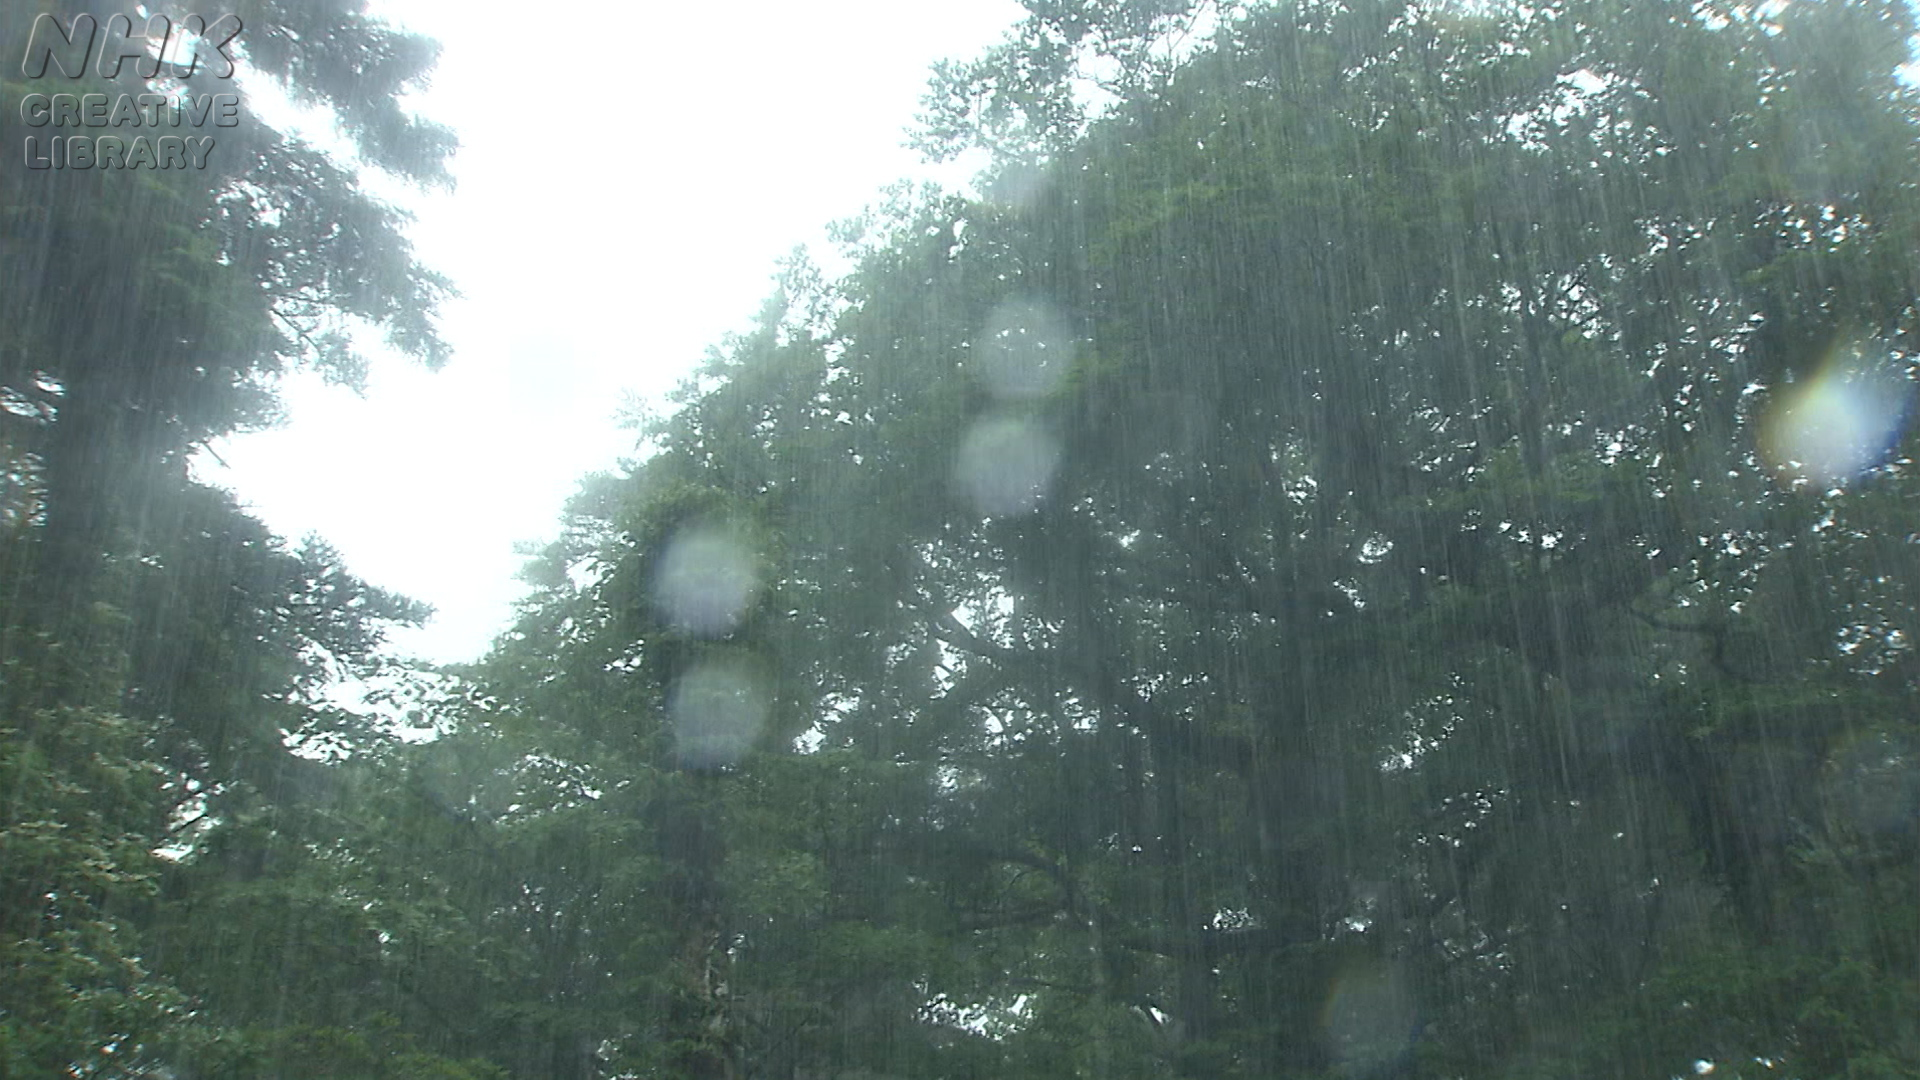
\includegraphics[width = 5cm]{./fig/sample.jpg}}{./movie/sample.mp4}
	\end{frame}
\end{document}